%%%%%%%%%%%%%%%%%%%%%%%%%%%%%%%%%%%%%%%%%
%  My documentation report
%  Objetive: Explain what I did and how, so someone can continue with the investigation
%
% Important note:
% Chapter heading images should have a 2:1 width:height ratio,
% e.g. 920px width and 460px height.
%
%%%%%%%%%%%%%%%%%%%%%%%%%%%%%%%%%%%%%%%%%

%----------------------------------------------------------------------------------------
%	PACKAGES AND OTHER DOCUMENT CONFIGURATIONS
%----------------------------------------------------------------------------------------

\documentclass[11pt,fleqn]{book} % Default font size and left-justified equations

\usepackage[top=3cm,bottom=3cm,left=3.2cm,right=3.2cm,headsep=10pt,letterpaper]{geometry} % Page margins

\usepackage{xcolor} % Required for specifying colors by name
\definecolor{ocre}{RGB}{52,177,201} % Define the orange color used for highlighting throughout the book

% Font Settings
\usepackage{avant} % Use the Avantgarde font for headings
%\usepackage{times} % Use the Times font for headings
\usepackage{mathptmx} % Use the Adobe Times Roman as the default text font together with math symbols from the Sym­bol, Chancery and Com­puter Modern fonts

\usepackage{microtype} % Slightly tweak font spacing for aesthetics
\usepackage[utf8]{inputenc} % Required for including letters with accents
\usepackage[T1]{fontenc} % Use 8-bit encoding that has 256 glyphs

%Tables
\usepackage{tabularx}
\usepackage{longtable,tabu}

% Bibliography
\usepackage[style=alphabetic,sorting=nyt,sortcites=true,autopunct=true,babel=hyphen,hyperref=true,abbreviate=false,backref=true,backend=biber]{biblatex}
\addbibresource{bibliography.bib} % BibTeX bibliography file
\defbibheading{bibempty}{}

\input{structure} % Insert the commands.tex file which contains the majority of the structure behind the template

\begin{document}

%----------------------------------------------------------------------------------------
%	TITLE PAGE
%----------------------------------------------------------------------------------------

\begingroup
\thispagestyle{empty}
\AddToShipoutPicture*{\put(0,0){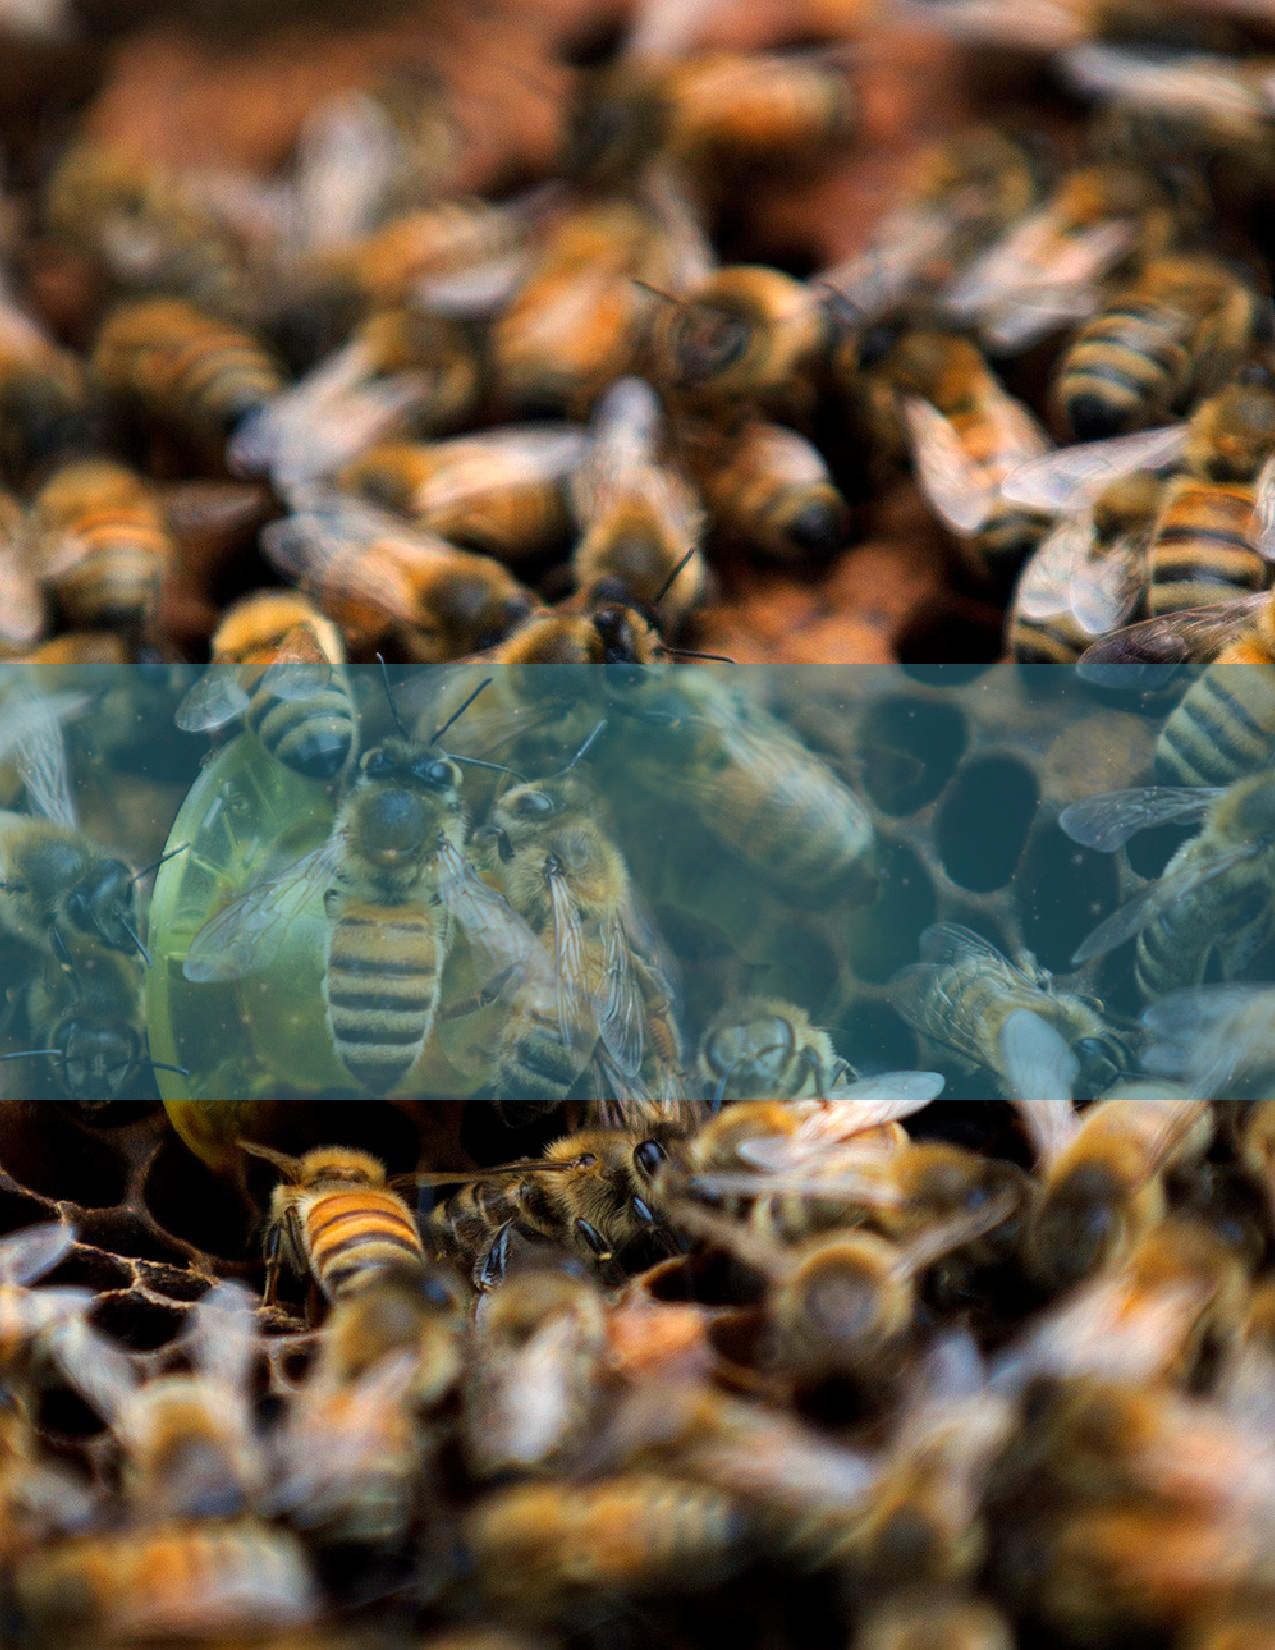
\includegraphics[scale=1.25]{cover}}} % Image background
\centering
\vspace*{4cm}
\par\normalfont\fontsize{35}{35}\sffamily\selectfont
\textbf{\color{white}Data Mining for Bee Micro-sensors}\\
{\Huge\color{white} Laboratorio Nacional de Análisis y Síntesis Ecológica}\par % Book title
\vspace*{0.2cm}
%Add all the collaborators
{\LARGE\color{white} Framework Developed by Ulises Olivares}\par % Author name
\endgroup

%----------------------------------------------------------------------------------------
%	COPYRIGHT PAGE
%----------------------------------------------------------------------------------------

\newpage
~\vfill
\thispagestyle{empty}

%\noindent Copyright \copyright\ 2014 Andrea Hidalgo\\ % Copyright notice

\noindent \textsc{High Performance Computing applied to biological sciences, Universidad Nacional Autónoma de México - Escuela Nacional de de Estudios Superiores Unidad Morelia - Laboratorio Nacional de Análisis y Síntesis Ecológica }\\

\noindent  This work was supported by grants from Consejo Nacional de Ciencia y Tecnología (CONACyT: Laboratorio Nacional de Análisis y Síntesis Ecológica U-3-2015-2-250996, CONACYT and CONACyT: Propuesta para eldesarrollo de una infraestructura tecnológica para lacreación de repositorios masivos de datos biológicos con fines de conservación y análisis de información I0028-2015-02-271432, CONACYT).\\ % License information

\noindent \textit{First release, April 2017} % Printing/edition date

%----------------------------------------------------------------------------------------
%	TABLE OF CONTENTS
%----------------------------------------------------------------------------------------

\chapterimage{head1.jpg} % Table of contents heading image

\pagestyle{empty} % No headers

\tableofcontents % Print the table of contents itself

%\cleardoublepage % Forces the first chapter to start on an odd page so it's on the right

\pagestyle{fancy} % Print headers again

%----------------------------------------------------------------------------------------
%	CHAPTER 1
%----------------------------------------------------------------------------------------
\chapterimage{head2.jpg} % Chapter heading image

\chapter{Analysis of the Hives' Activity}

%INSERT_CONTENT_HERE
\normalsize%
\section*{Introduction}%
The main propose of this document  is to show a concise report about the activity of bees and behavior in a specific period of time. This report also shows a complete analysis of the most active hours.\newline%
\newline%
Tis report corresponds to a period of time of 62 day(s). From 2016{-}08{-}24 to 2016{-}11{-}24. During this period of time, a total amount of 22305 lectures were registered from 75 different bees. There exist a total of 22 non{-}active days. We define an 'active day' if there is more than one observation. (see Figure1.1).\newline%
\newline%
%


\begin{figure}[h!]%
\centering%
\includegraphics[width=315px]{chartNumLectures.png}%
\caption{Days with and without Empty Reads}%
\end{figure}

%
\subsection*{Activity per day}%
This section addresses the analysis of the activity per day%


\begin{figure}[h!]%
\centering%
\includegraphics[width=400px]{observationsPerday.png}%
\caption{Number of Observations per Day}%
\end{figure}

%
\begin{longtabu}{| c | c | c | c |}%
\hline%
Day&Date&\# Observations&\# Bees per day\\%
\hline%
1&2016{-}08{-}24&35&8\\%
\hline%
2&2016{-}08{-}25&7&3\\%
\hline%
3&2016{-}08{-}26&7&2\\%
\hline%
4&2016{-}08{-}27&86&4\\%
\hline%
5&2016{-}08{-}29&33&2\\%
\hline%
6&2016{-}08{-}30&3&1\\%
\hline%
7&2016{-}08{-}31&2&1\\%
\hline%
8&2016{-}09{-}02&8&1\\%
\hline%
9&2016{-}09{-}05&2&1\\%
\hline%
10&2016{-}09{-}08&3&1\\%
\hline%
11&2016{-}09{-}09&25&6\\%
\hline%
12&2016{-}09{-}10&5345&3\\%
\hline%
13&2016{-}09{-}11&189&12\\%
\hline%
14&2016{-}09{-}12&94&4\\%
\hline%
15&2016{-}09{-}13&82&12\\%
\hline%
16&2016{-}09{-}14&135&10\\%
\hline%
17&2016{-}09{-}15&160&6\\%
\hline%
18&2016{-}09{-}16&30&7\\%
\hline%
19&2016{-}09{-}17&52&12\\%
\hline%
20&2016{-}09{-}18&88&6\\%
\hline%
21&2016{-}09{-}19&131&13\\%
\hline%
22&2016{-}09{-}20&77&5\\%
\hline%
23&2016{-}09{-}21&203&11\\%
\hline%
24&2016{-}09{-}22&92&5\\%
\hline%
25&2016{-}09{-}23&51&8\\%
\hline%
26&2016{-}09{-}24&257&11\\%
\hline%
27&2016{-}09{-}25&1253&6\\%
\hline%
28&2016{-}09{-}26&39&9\\%
\hline%
29&2016{-}09{-}27&123&6\\%
\hline%
30&2016{-}09{-}28&90&9\\%
\hline%
31&2016{-}09{-}29&9109&19\\%
\hline%
32&2016{-}09{-}30&239&18\\%
\hline%
33&2016{-}10{-}01&122&12\\%
\hline%
34&2016{-}10{-}02&877&17\\%
\hline%
35&2016{-}10{-}03&240&14\\%
\hline%
36&2016{-}10{-}04&866&14\\%
\hline%
37&2016{-}10{-}05&393&12\\%
\hline%
38&2016{-}10{-}06&345&10\\%
\hline%
39&2016{-}10{-}07&107&8\\%
\hline%
40&2016{-}10{-}08&83&8\\%
\hline%
41&2016{-}10{-}09&49&8\\%
\hline%
42&2016{-}10{-}10&36&5\\%
\hline%
43&2016{-}10{-}11&36&5\\%
\hline%
44&2016{-}10{-}12&118&6\\%
\hline%
45&2016{-}10{-}13&23&2\\%
\hline%
46&2016{-}10{-}14&28&4\\%
\hline%
47&2016{-}10{-}15&24&4\\%
\hline%
48&2016{-}10{-}16&25&3\\%
\hline%
49&2016{-}10{-}17&29&2\\%
\hline%
50&2016{-}10{-}18&28&2\\%
\hline%
51&2016{-}11{-}13&279&9\\%
\hline%
52&2016{-}11{-}14&49&6\\%
\hline%
53&2016{-}11{-}15&60&9\\%
\hline%
54&2016{-}11{-}16&42&7\\%
\hline%
55&2016{-}11{-}17&63&10\\%
\hline%
56&2016{-}11{-}18&52&8\\%
\hline%
57&2016{-}11{-}19&63&6\\%
\hline%
58&2016{-}11{-}20&39&10\\%
\hline%
59&2016{-}11{-}21&40&6\\%
\hline%
60&2016{-}11{-}22&62&11\\%
\hline%
61&2016{-}11{-}23&30&6\\%
\hline%
62&2016{-}11{-}24&47&7\\%
\hline%
\hline%
{-}{-}&Average&359&7\\%
\hline%
\hline%
\end{longtabu}

%
\subsection*{Bee Life Cycle}%
In this section is analyzed the Life Cycle of each bee in the hive%
\begin{longtabu}{| c | c | c |}%
\hline%
\hline%
Register&Bee ID&Life Cycle in Days\\%
\hline%
\hline%
1&0034&1\\%
\hline%
2&0039&1\\%
\hline%
3&0044&1\\%
\hline%
4&0127&23\\%
\hline%
5&0148&1\\%
\hline%
6&0182&1\\%
\hline%
7&0022&1\\%
\hline%
8&0029&4\\%
\hline%
9&0036&3\\%
\hline%
10&0038&1\\%
\hline%
11&0044&2\\%
\hline%
12&0053&1\\%
\hline%
13&0065&55\\%
\hline%
14&0073&1\\%
\hline%
15&0088&1\\%
\hline%
16&0090&1\\%
\hline%
17&0100&4\\%
\hline%
18&0106&5\\%
\hline%
19&0107&4\\%
\hline%
20&0108&18\\%
\hline%
21&0110&17\\%
\hline%
22&0113&2\\%
\hline%
23&0114&15\\%
\hline%
24&0115&22\\%
\hline%
25&0122&12\\%
\hline%
26&0131&17\\%
\hline%
27&0132&11\\%
\hline%
28&0136&5\\%
\hline%
29&0143&26\\%
\hline%
30&0148&7\\%
\hline%
31&0153&19\\%
\hline%
32&0161&26\\%
\hline%
33&0170&2\\%
\hline%
34&0176&21\\%
\hline%
35&0177&1\\%
\hline%
36&0183&36\\%
\hline%
37&0186&32\\%
\hline%
38&0189&1\\%
\hline%
39&0202&1\\%
\hline%
40&0210&2\\%
\hline%
41&0211&10\\%
\hline%
42&0222&1\\%
\hline%
43&0232&1\\%
\hline%
44&0244&17\\%
\hline%
45&0246&1\\%
\hline%
46&0250&1\\%
\hline%
47&0255&3\\%
\hline%
48&0259&20\\%
\hline%
49&0260&1\\%
\hline%
50&0262&20\\%
\hline%
51&0263&10\\%
\hline%
52&0272&1\\%
\hline%
53&0273&1\\%
\hline%
54&0278&1\\%
\hline%
55&0284&1\\%
\hline%
56&0288&1\\%
\hline%
57&0292&1\\%
\hline%
58&0300&6\\%
\hline%
59&0356&11\\%
\hline%
60&0357&7\\%
\hline%
61&0385&1\\%
\hline%
62&0406&2\\%
\hline%
63&0407&11\\%
\hline%
64&0417&10\\%
\hline%
65&0431&12\\%
\hline%
66&0433&8\\%
\hline%
67&0434&8\\%
\hline%
68&0456&10\\%
\hline%
69&0459&5\\%
\hline%
70&0465&12\\%
\hline%
71&0466&12\\%
\hline%
72&0469&1\\%
\hline%
73&0482&10\\%
\hline%
74&0490&10\\%
\hline%
75&0499&8\\%
\hline%
\hline%
{-}{-}&Average&8\\%
\hline%
\hline%
\end{longtabu}%


\begin{figure}[h!]%
\centering%
\includegraphics[width=400px]{differentBeesPerday.png}%
\caption{Different Bees Per Day}%
\end{figure}

%


\begin{figure}[h!]%
\centering%
\includegraphics[width=400px]{beeLifeCycle.png}%
\caption{Bee Life cycle in days}%
\end{figure}

%


\begin{figure}[h!]%
\centering%
\includegraphics[width=400px]{pieBeeLifeCycle.png}%
\caption{Bee Life cycle in days}%
\end{figure}

%
\subsection*{Analysis of Activity per Hour}%


\begin{figure}[h!]%
\centering%
\includegraphics[width=400px]{histogram.png}%
\caption{Histogram of frequencies per hour}%
\end{figure}

%


\begin{figure}[h!]%
\centering%
\includegraphics[width=400px]{histogramStd.png}%
\caption{Histogram of frequencies per hour. It includes standard deviation}%
\end{figure}


\end{document}